\documentclass[12pt]{article}
% !TEX root = transfer.tex

\usepackage[utf8]{inputenc}
\usepackage[T1]{fontenc}
\usepackage{lmodern}
\usepackage{mathtools}
% \usepackage{xcolor}
\usepackage[hidelinks]{hyperref}
\usepackage{algorithm}
\usepackage[noend]{algpseudocode}
% \usepackage{algorithmicx}
\usepackage{graphicx}
\usepackage{animate}
\usepackage{booktabs}
\usepackage{tabulary}
\usepackage{rotating}
\usepackage{natbib}

\usepackage{dsfont}

\usepackage{tikz}
\usetikzlibrary{bayesnet}

\usepackage{todonotes}
\presetkeys{todonotes}{inline}{}

% Change font to Times New Roman
% \usepackage{newtxtext}

\usepackage{amsfonts}
\usepackage{amssymb,amstext,amsmath, amsthm}

% Algorithm stuff
\makeatletter
\newcounter{algorithmbis}
\setcounter{algorithmbis}{0}
\renewcommand{\thealgorithmbis}{\arabic{algorithmbis}}
\def\algorithmbis{\@ifnextchar[{\@algorithmbisa}{\@algorithmbisb}}
\def\@algorithmbisa[#1]{%
  \refstepcounter{algorithmbis}
  \trivlist
  \leftmargin\z@
  \itemindent\z@
  \labelsep\z@
  \item[\parbox{\textwidth}{%
    \hrule
    \hrule
    \noindent\strut\textbf{Algorithm \thealgorithmbis} #1
    \hrule
  }]\hfil\vskip0em%
}
% \newcommand*{\oldeqref}{}
% \let\oldeqref\eqref
% \renewcommand*{\eqref}[1]{%
%   \begingroup
%     \hypersetup{
%       linkcolor=linkequation,
%       linkbordercolor=linkequation,
%     }%
%     \oldeqref{#1}%
%   \endgroup
% }
\def\@algorithmbisb{\@algorithmbisa[]}
\def\endalgorithmbis{\hfil\vskip-1em\hrule\endtrivlist}
\makeatother

% Math stuff
% \DeclareMathOperator*{\argmin}{arg\,min}
% \DeclareMathOperator*{\argmax}{arg\,max}
% \DeclareMathOperator{\Bin}{Bin}
% \DeclareMathOperator{\Ber}{Ber}
% \DeclareMathOperator{\Beta}{Beta}
% \DeclareMathOperator{\BetaBin}{BetaBin}
% \DeclareMathOperator{\Cat}{Cat}
% \DeclareMathOperator{\Dir}{Dir}
% \DeclareMathOperator{\DirMult}{DirMult}
% \DeclareMathOperator{\Mult}{Mult}
% \DeclareMathOperator{\Poi}{Poi}
% \DeclareMathOperator{\Gammadist}{Gamma}
% \DeclareMathOperator{\NB}{NB}
% \DeclareMathOperator{\Unif}{Unif}
% \DeclareMathOperator{\Pareto}{Pareto}
% \DeclareMathOperator{\Gauss}{\mathcal N}
% \DeclareMathOperator{\E}{\mathbb{E}}
% \DeclareMathOperator{\var}{\mathrm{var}}
% \DeclareMathOperator{\cov}{\mathrm{cov}}
% \DeclareMathOperator{\grad}{\mathrm{grad}}
% \newcommand*\mean[1]{\bar{#1}}
% \DeclareMathOperator{\diag}{diag}
% \DeclareMathOperator{\KL}{KL}
% \DeclareMathOperator{\Tr}{Tr}
% \DeclareMathOperator{\DP}{DP}
% \DeclareMathOperator{\GP}{GP}
% \DeclareMathOperator{\GEM}{GEM}
% \DeclareMathOperator{\I}{\mathbb I}
% \DeclareMathOperator{\pa}{pa}
\let\oldemptyset\emptyset
\let\emptyset\varnothing
\newcommand{\at}[2][]{#1|_{#2}}
\newcommand{\given}{|}

% bold vectors
\renewcommand{\vec}[1]{\boldsymbol{\mathbf{#1}}}

% Theorem, proofs, etc.
\usepackage{amsthm}
\usepackage{thmtools}
\makeatletter
\def\thm@space@setup{%
  \thm@preskip=\parskip \thm@postskip=0pt
}
\makeatother
\theoremstyle{definition}
% \newtheorem{definition}{Definition}[section]
\declaretheorem[qed=$\triangle$,numberwithin=section]{definition}
\newtheorem{theorem}{Theorem}[section]
\newtheorem{proposition}{Proposition}[section]
\newtheorem{claim}{Claim}[section]
% End with a triangle
\declaretheorem[qed=$\triangle$,sibling=definition]{example}

% Double spacing
\usepackage{setspace}
% \doublespacing

% Margins
\usepackage[margin=2cm,a4paper]{geometry}

% No indent, but skip paragraphs
\usepackage[parfill]{parskip}

% 1st, 2nd, 3rd, 4th, etc.
\usepackage[super]{nth}

% including code
\usepackage{listing}
% \usepackage{listings}
\usepackage{color}
\usepackage{xcolor}
\definecolor{blue}{rgb}{0,0.3,0.7}
\definecolor{red}{rgb}{0.60,0.0,0.0}
\definecolor{purple}{rgb}{0.5,0,0.7}
\definecolor{cyan}{rgb}{0.0,0.6,0.5}
\definecolor{gray}{rgb}{0.4,0.4,0.4}

\lstdefinelanguage{scheme}
{sensitive, %
 alsoletter={:,-,+,*,?,/,!,>,<}, %
 morecomment=[l]{;}, %
}[comments]

% listings definition for Anglican programming language
\lstdefinelanguage{anglican}%
{% empty (strings and keywords)
 morekeywords=[1]{},
 % clojure declarations
 morekeywords=[2]{%
   def, def-, defn, defn-, defmacro, defmulti, defmethod, %
   defstruct, defonce, declare, definline, definterface, %
   defprotocol, defrecord, defstruct, deftype, defproject, ns, %
 }, %
 % clojure macros and special forms
 morekeywords=[3]{->, ->>, .., amap, and, areduce, as->, assert, binding, %
   bound-fn, case, comment, cond, cond->, cond->>, condp, declare, definline, %
   definterface, defmacro, defmethod, defmulti, defn, defn-, defonce, %
   defprotocol, defrecord, defstruct, deftype, delay, doseq, dosync, dotimes, %
   doto, extend-protocol, extend-type, fn, for, future, gen-class, %
   gen-interface, if, if-let, if-not, if-some, import, io!, lazy-cat, lazy-seq, let, %
   letfn, locking, loop, memfn, ns, or, proxy, proxy-super, pvalues, %
   recur, refer-clojure, reify, some->, some->>, sync, time, when, when-first, %
   when-let, when-not, when-some, while, with-bindings, with-in-str, %
   with-loading-context, with-local-vars, with-open, with-out-str, %
   with-precision, with-redefs, else}, %
  % clojure functions
  morekeywords=[4]{*, *', +, +', -, -', ->ArrayChunk, ->Vec, ->VecNode, %
    ->VecSeq, -cache-protocol-fn, -reset-methods, /, <, <=, =, ==, >, >=, %
    accessor, aclone, add-classpath, add-watch, agent, agent-error, %
    agent-errors, aget, alength, alias, all-ns, alter, alter-meta!, %
    alter-var-root, ancestors, apply, array-map, aset, aset-boolean, aset-byte, %
    aset-char, aset-double, aset-float, aset-int, aset-long, aset-short, assoc, %
    assoc!, assoc-in, associative?, atom, await, await-for, await1, bases, bean, %
    bigdec, bigint, biginteger, bit-and, bit-and-not, bit-clear, bit-flip, %
    bit-not, bit-or, bit-set, bit-shift-left, bit-shift-right, bit-test, %
    bit-xor, boolean, boolean-array, booleans, bound-fn*, bound?, butlast, byte, %
    byte-array, bytes, cast, char, char-array, char?, chars, chunk, %
    chunk-append, chunk-buffer, chunk-cons, chunk-first, chunk-next, chunk-rest, %
    chunked-seq?, class, class?, clear-agent-errors, clojure-version, coll?, %
    commute, comp, comparator, compare, compare-and-set!, compile, complement, %
    concat, conj, conj!, cons, constantly, construct-proxy, contains?, count, %
    counted?, create-ns, create-struct, cycle, dec, dec', decimal?, delay?, %
    deliver, denominator, deref, derive, descendants, destructure, disj, disj!, %
    dissoc, dissoc!, distinct, distinct?, doall, dorun, double, double-array, %
    doubles, drop, drop-last, drop-while, empty, empty?, ensure, %
    enumeration-seq, error-handler, error-mode, eval, even?, every-pred, every?, %
    ex-data, ex-info, extend, extenders, extends?, false?, ffirst, file-seq, %
    filter, filter-ns-publics, filterv, find, find-keyword, find-ns, %
    find-protocol-impl, find-protocol-method, find-var, first, flatten, float, %
    float-array, float?, floats, flush, fn?, fnext, fnil, force, format, %
    frequencies, future-call, future-cancel, future-cancelled?, future-done?, %
    future?, gensym, get, get-in, get-method, get-proxy-class, %
    get-thread-bindings, get-validator, group-by, hash, hash-combine, hash-map, %
    hash-ordered-coll, hash-set, hash-unordered-coll, identical?, identity, %
    ifn?, in-ns, inc, inc', init-proxy, instance?, int, int-array, integer?, %
    interleave, intern, interpose, into, into-array, ints, isa?, iterate, %
    iterator-seq, juxt, keep, keep-indexed, key, keys, keyword, keyword?, last, %
    line-seq, list, list*, list?, load, load-file, load-reader, load-string, %
    loaded-libs, long, long-array, longs, macroexpand, macroexpand-1, %
    make-array, make-hierarchy, map, map-indexed, map?, mapcat, mapv, max, %
    max-key, memoize, merge, merge-with, meta, method-sig, methods, min, %
    min-key, mix-collection-hash, mod, munge, name, namespace, namespace-munge, %
    neg?, newline, next, nfirst, nil?, nnext, not, not-any?, not-empty, %
    not-every?, not=, ns-aliases, ns-functions, ns-imports, ns-interns, %
    ns-macros, ns-map, ns-name, ns-publics, ns-refers, ns-resolve, ns-unalias, %
    ns-unmap, nth, nthnext, nthrest, num, number?, numerator, object-array, %
    odd?, parents, partial, partition, partition-all, partition-by, pcalls, %
    peek, persistent!, pmap, pop, pop!, pop-thread-bindings, pos?, pr, pr-str, %
    prefer-method, prefers, print, print-ctor, print-simple, print-str, printf, %
    println, println-str, prn, prn-str, promise, proxy-call-with-super, %
    proxy-mappings, proxy-name, push-thread-bindings, quot, rand, rand-int, %
    rand-nth, range, ratio?, rational?, rationalize, re-find, re-groups, %
    re-matcher, re-matches, re-pattern, re-seq, read, read-line, read-string, %
    realized?, record?, reduce, reduce-kv, reduced, reduced?, reductions, ref, %
    ref-history-count, ref-max-history, ref-min-history, ref-set, refer, %
    release-pending-sends, rem, remove, remove-all-methods, remove-method, %
    remove-ns, remove-watch, repeat, repeatedly, replace, replicate, require, %
    reset!, reset-meta!, resolve, rest, restart-agent, resultset-seq, reverse, %
    reversible?, rseq, rsubseq, satisfies?, second, select-keys, send, send-off, %
    send-via, seq, seq?, seque, sequence, sequential?, set, %
    set-agent-send-executor!, set-agent-send-off-executor!, set-error-handler!, %
    set-error-mode!, set-validator!, set?, short, short-array, shorts, shuffle, %
    shutdown-agents, slurp, some, some-fn, some?, sort, sort-by, sorted-map, %
    sorted-map-by, sorted-set, sorted-set-by, sorted?, special-symbol?, spit, %
    split-at, split-with, str, string?, struct, struct-map, subs, subseq, %
    subvec, supers, swap!, symbol, symbol?, take, take-last, take-nth, %
    take-while, test, the-ns, thread-bound?, to-array, to-array-2d, trampoline, %
    transient, tree-seq, true?, type, unchecked-add, unchecked-add-int, %
    unchecked-byte, unchecked-char, unchecked-dec, unchecked-dec-int, %
    unchecked-divide-int, unchecked-double, unchecked-float, unchecked-inc, %
    unchecked-inc-int, unchecked-int, unchecked-long, unchecked-multiply, %
    unchecked-multiply-int, unchecked-negate, unchecked-negate-int, %
    unchecked-remainder-int, unchecked-short, unchecked-subtract, %
    unchecked-subtract-int, underive, unsigned-bit-shift-right, update-in, %
    update-proxy, use, val, vals, var-get, var-set, var?, vary-meta, vec, %
    vector, vector-of, vector?, with-bindings*, with-meta, with-redefs-fn, %
    xml-seq, zero?, zipmap}, %
  % anglican declarations
  morekeywords=[5]{def-cps-fn, defanglican, defm, defquery, defun, defproc, defdist}, %
  % anglican macros
  morekeywords=[6]{cps-fn, fm, lambda, query, with-primitive-procedures}, %
  % anglican functions
  morekeywords=[7]{%
    % anglican.core
    doquery, %
    % anglican.emit
    conditional, %
    % anglican.inference
    collect-by, equalize, exec, infer, log-marginal, print-predicts, %
    rand, rand-int, rand-nth, rand-roulette, stripdown, warmup, %
    % anglican.runtime
    ->CRP-process, ->DP-process, ->GP-process, %
    ->bernoulli-distribution, ->beta-distribution, ->binomial-distribution, %
    ->categorical-crp-distribution, ->categorical-distribution, %
    ->categorical-dp-distribution, ->chi-squared-distribution, %
    ->dirichlet-distribution, ->discrete-distribution, %
    ->exponential-distribution, ->flip-distribution, ->gamma-distribution, %
    ->mvn-distribution, ->normal-distribution, ->poisson-distribution, %
    ->sample, ->observe, sample*, observe*, %
    ->uniform-continuous-distribution, ->uniform-discrete-distribution, %
    ->wishart-distribution, CRP, DP, GP, abs, absorb, acos, asin, atan, %
    bernoulli, beta, binomial, categorical, categorical-crp, categorical-dp, %
    cbrt, ceil, chi-squared, cos, cosh, cov, dirichlet, discrete, exp, %
    exponential, flip, floor, gamma, gen-matrix, log, log-gamma-fn, %
    log-mv-gamma-fn, log-sum-exp, map->CRP-process, map->DP-process, %
    map->GP-process, map->bernoulli-distribution, map->beta-distribution, %
    map->binomial-distribution, map->categorical-crp-distribution, %
    map->categorical-distribution, map->categorical-dp-distribution, %
    map->chi-squared-distribution, map->dirichlet-distribution, %
    map->discrete-distribution, map->exponential-distribution, %
    map->flip-distribution, map->gamma-distribution, map->mvn-distribution, %
    map->normal-distribution, map->poisson-distribution, %
    map->uniform-continuous-distribution, map->uniform-discrete-distribution, %
    map->wishart-distribution, mvn, normal, poisson, pow, produce, %
    rint, round, signum, sin, sinh, sqrt, tag, tan, tanh, transform-sample, %
    uniform-continuous, uniform-discrete, wishart, uniform, %
    % anglican.state
    add-log-weight, add-predict, clear-predicts, get-log-weight, %
    get-mem, get-predicts, in-mem?, set-log-weight, set-mem, %     
  }, %
  % anglican special forms
  morekeywords=[8]{factor, mem, observe, predict, retrieve, sample, store}, %
  sensitive, %
  alsoletter={:,-,+,*,?,/,!,>,<,.}, %
  morecomment=[l][\color{gray}]{;}, %
  morestring=[b]", %
  %keywordsprefix=:, %
}[keywords,comments,strings]
 
\lstset{
  language=anglican,
  basicstyle=\ttfamily,
  commentstyle=\em\color{gray},
  % keywords and strings
  keywordstyle=[1]\color{red},
  stringstyle=\color{gray},
  % clojure declarations
  keywordstyle=[2]\color{purple}\bfseries,
  % clojure macros and special forms
  keywordstyle=[3]\color{red}\bfseries,
  % clojure functions
  keywordstyle=[4]\color{cyan}\bfseries,
  % anglican declarations
  keywordstyle=[5]\color{purple}\bfseries,
  % anglican macros
  keywordstyle=[6]\color{red}\bfseries,
  % anglican functions
  keywordstyle=[7]\color{cyan}\bfseries,
  % anglican inference forms 
  keywordstyle=[8]\color{blue}\bfseries
}

% \lstdefinestyle{default}{language=Anglican,basicstyle=\ttfamily\small, columns=flexible, showstringspaces=false}

\usepackage{enumitem}
\setlist{noitemsep, topsep=-5pt}

% verbatim font size
% \makeatletter
%   \def\verbatim{\huge\@verbatim \frenchspacing\@vobeyspaces \@xverbatim}
% \makeatother

% lorem ipsum
\usepackage{lipsum}

% subfig
\usepackage{subcaption}

% for titlepage
\newcommand{\HRule}{\rule{\linewidth}{0.5mm}}

% clojure listings
% \lstdefinelanguage{clojure}%
% {morekeywords={*,*1,*2,*3,*agent*,*allow-unresolved-vars*,*assert*,*clojure-version*,*command-line-args*,%
% *compile-files*,*compile-path*,*e,*err*,*file*,*flush-on-newline*,*in*,*macro-meta*,%
% *math-context*,*ns*,*out*,*print-dup*,*print-length*,*print-level*,*print-meta*,*print-readably*,%
% *read-eval*,*source-path*,*use-context-classloader*,*warn-on-reflection*,+,-,->,->>,..,/,:else,%
% <,<=,=,==,>,>=,@,accessor,aclone,add-classpath,add-watch,agent,agent-errors,aget,alength,alias,%
% all-ns,alter,alter-meta!,alter-var-root,amap,ancestors,and,apply,areduce,array-map,aset,%
% aset-boolean,aset-byte,aset-char,aset-double,aset-float,aset-int,aset-long,aset-short,assert,%
% assoc,assoc!,assoc-in,associative?,atom,await,await-for,await1,bases,bean,bigdec,bigint,binding,%
% bit-and,bit-and-not,bit-clear,bit-flip,bit-not,bit-or,bit-set,bit-shift-left,bit-shift-right,%
% bit-test,bit-xor,boolean,boolean-array,booleans,bound-fn,bound-fn*,butlast,byte,byte-array,%
% bytes,cast,char,char-array,char-escape-string,char-name-string,char?,chars,chunk,chunk-append,%
% chunk-buffer,chunk-cons,chunk-first,chunk-next,chunk-rest,chunked-seq?,class,class?,%
% clear-agent-errors,clojure-version,coll?,comment,commute,comp,comparator,compare,compare-and-set!,%
% compile,complement,concat,cond,condp,conj,conj!,cons,constantly,construct-proxy,contains?,count,%
% counted?,create-ns,create-struct,cycle,dec,decimal?,declare,def,definline,defmacro,defmethod,%
% defmulti,defn,defn-,defonce,defprotocol,defstruct,deftype,delay,delay?,deliver,deref,derive,%
% descendants,destructure,disj,disj!,dissoc,dissoc!,distinct,distinct?,do,do-template,doall,doc,%
% dorun,doseq,dosync,dotimes,doto,double,double-array,doubles,drop,drop-last,drop-while,empty,empty?,%
% ensure,enumeration-seq,eval,even?,every?,false,false?,ffirst,file-seq,filter,finally,find,find-doc,%
% find-ns,find-var,first,float,float-array,float?,floats,flush,fn,fn?,fnext,for,force,format,future,%
% future-call,future-cancel,future-cancelled?,future-done?,future?,gen-class,gen-interface,gensym,%
% get,get-in,get-method,get-proxy-class,get-thread-bindings,get-validator,hash,hash-map,hash-set,%
% identical?,identity,if,if-let,if-not,ifn?,import,in-ns,inc,init-proxy,instance?,int,int-array,%
% integer?,interleave,intern,interpose,into,into-array,ints,io!,isa?,iterate,iterator-seq,juxt,%
% key,keys,keyword,keyword?,last,lazy-cat,lazy-seq,let,letfn,line-seq,list,list*,list?,load,load-file,%
% load-reader,load-string,loaded-libs,locking,long,long-array,longs,loop,macroexpand,macroexpand-1,%
% make-array,make-hierarchy,map,map?,mapcat,max,max-key,memfn,memoize,merge,merge-with,meta,%
% method-sig,methods,min,min-key,mod,monitor-enter,monitor-exit,name,namespace,neg?,new,newline,%
% next,nfirst,nil,nil?,nnext,not,not-any?,not-empty,not-every?,not=,ns,ns-aliases,ns-imports,%
% ns-interns,ns-map,ns-name,ns-publics,ns-refers,ns-resolve,ns-unalias,ns-unmap,nth,nthnext,num,%
% number?,odd?,or,parents,partial,partition,pcalls,peek,persistent!,pmap,pop,pop!,pop-thread-bindings,%
% pos?,pr,pr-str,prefer-method,prefers,primitives-classnames,print,print-ctor,print-doc,print-dup,%
% print-method,print-namespace-doc,print-simple,print-special-doc,print-str,printf,println,println-str,%
% prn,prn-str,promise,proxy,proxy-call-with-super,proxy-mappings,proxy-name,proxy-super,%
% push-thread-bindings,pvalues,quot,rand,rand-int,range,ratio?,rational?,rationalize,re-find,%
% re-groups,re-matcher,re-matches,re-pattern,re-seq,read,read-line,read-string,recur,reduce,ref,%
% ref-history-count,ref-max-history,ref-min-history,ref-set,refer,refer-clojure,reify,%
% release-pending-sends,rem,remove,remove-method,remove-ns,remove-watch,repeat,repeatedly,%
% replace,replicate,require,reset!,reset-meta!,resolve,rest,resultset-seq,reverse,reversible?,%
% rseq,rsubseq,second,select-keys,send,send-off,seq,seq?,seque,sequence,sequential?,set,set!,%
% set-validator!,set?,short,short-array,shorts,shutdown-agents,slurp,some,sort,sort-by,sorted-map,%
% sorted-map-by,sorted-set,sorted-set-by,sorted?,special-form-anchor,special-symbol?,split-at,%
% split-with,str,stream?,string?,struct,struct-map,subs,subseq,subvec,supers,swap!,symbol,symbol?,%
% sync,syntax-symbol-anchor,take,take-last,take-nth,take-while,test,the-ns,throw,time,to-array,%
% to-array-2d,trampoline,transient,tree-seq,true,true?,try,type,unchecked-add,unchecked-dec,%
% unchecked-divide,unchecked-inc,unchecked-multiply,unchecked-negate,unchecked-remainder,%
% unchecked-subtract,underive,unquote,unquote-splicing,update-in,update-proxy,use,val,vals,%
% var,var-get,var-set,var?,vary-meta,vec,vector,vector?,when,when-first,when-let,when-not,%
% while,with-bindings,with-bindings*,with-in-str,with-loading-context,with-local-vars,%
% with-meta,with-open,with-out-str,with-precision,xml-seq,zero?,zipmap
% },%
%    sensitive,% ???
%    alsodigit=-,%
%    morecomment=[l];,%
%    morestring=[b]"%
%   }[keywords,comments,strings]%

% for including pdfs
\usepackage{pdfpages}


% custom abbreviations
\usepackage{abbreviations}

\usepackage{listings}
\usepackage{color}
\usepackage{xcolor}
\usepackage{textcomp}
\usepackage{xspace}
\definecolor{darkgreenClj}{rgb}{0.25,.5,0.25}
\definecolor{blueClj}{rgb}{0,0.33,0.66}
\definecolor{redClj}{rgb}{0.66,0.0,0.0}
\definecolor{purpleClj}{rgb}{0.33,0,0.66}
\definecolor{cyanClj}{rgb}{0.0,0.5,0.5}
\definecolor{orangeClj}{rgb}{0.75,0.35,0.0}
\definecolor{grayClj}{rgb}{0.4,0.4,0.4}
\lstset{ 
	language=Lisp, 
	basicstyle=\small\ttfamily,
	keywordstyle={}, 
	alsoletter={<-,->,:,*,/,?,+,-,/,>,<,=, &},
	commentstyle=\em \color{gray}, 
	frame=lines,
	%float=tbph,
	% captionpos=b,
	showstringspaces=false, 
	keywordstyle=[1]\bf\ttfamily\color{blueClj},
	keywords=[1]{BO,theta-best,bo-acquire,sample-initial-points,sample,observe,observe<-,predict,mem,store,retrieve,return,catch,throw,absorb,produce,with-primitive-procedures,conditional,result,log-marginal,mean,collect-results,empirical-mean,empirical-distribution,
		->sample,->observe,->result},
	keywordstyle=[2]\bf\ttfamily\color{redClj},
	keywords=[2]{if,let,letfn,loop,looppredict,recur,or,trampoline,assoc,argmax,count,cons,conj,case,
		do,first,fn,get,keys,lazy-seq,map,nth,mat/add,mat/div,print,reduce,repeat,repeatedly,rest,set,shape,take,vec,
		when,max,fn?,inc,sample*,observe*},
	keywordstyle=[3]\bf\ttfamily\color{cyanClj},
	keywords=[3]{dirichlet-discrete,exponential,flip,gamma,beta,mvn-niw,normal,uniform-continuous,distribution,factor,categorical,hand-strength,
		play-prior,simulate,abc-likelihood,student-t,dirichlet},
	keywordstyle=[4]\bf\ttfamily\color{purpleClj},
	keywords=[4]{defopt,defquery,doopt,doquery,query,defdist,infer,checkpoint,exec,defm,cps-of-expression,defint,
		defn,def,declare},
	keywordstyle=[5]\bf\ttfamily\color{orangeClj},
	keywords=[5]{:lmh,:ipmcmc,:war,:peace,:log-weight,:result,:id,:dist,:cont,:value,:state,:importance,:smc,:pgibbs,:fold,:bet,
		:number-of-particles},
	mathescape=true,
	stringstyle={},
	keywordstyle=[6]\bf\ttfamily\color{darkgreenClj},
	keywords=[6]{+,-,nil,>,<,*,/,=, &,->>,->},
	mathescape=true,
	stringstyle={},
} 
\lstnewenvironment{code}[2]{\lstset{caption=#1,label=#2}}{}


\begin{document}
% !TEX root = transfer.tex

\begin{titlepage}
\begin{center}

% Upper part of the page. The '~' is needed because \\
% only works if a paragraph has started.
~\\[2cm]

\textsc{\LARGE Transfer of Status Report}\\[2cm]


\includegraphics[width=0.3\textwidth]{title/oxford.pdf}\\[2cm]

\textsc{\Large University of Oxford}\\
\textsc{\Large Department of Engineering Science}\\[2cm]


% Author and supervisor
\begin{minipage}{0.4\textwidth}
\begin{flushleft} \large
\emph{Author:}\\
Adam Goli\'{n}ski\\
\text{}\\
\text{}
\end{flushleft}
\end{minipage}
\begin{minipage}{0.4\linewidth}
\begin{flushright} \large
\emph{Supervisors:} \\

Yee Whye Teh \\
Frank Wood \\
Michael Osborne
\end{flushright}
\end{minipage}

\vfill

% Bottom of the page
% {\large Michaelmas 2016} \\
{\large \today}

\end{center}
\end{titlepage}


% \title{Improving, Extending and Automating\\Amortized Probabilistic Inference and Data Compression}
\title{Advances in Probabilistic Inference and Data Compression using Deep Learning}
\date{}
\maketitle

\vspace{-50pt}


\section{Introduction}

This report consists of three parts:
\begin{itemize}
\item Description of the projects I have worked on and I intend to use for my thesis,
\item Planned steps to completion of my thesis,
\item The manuscript of my paper \emph{Amortized Monte Carlo Integration} published at ICML 2019.
\end{itemize}



\section{Progress towards the thesis}

Outside of the manuscript attached in the last part of this report,
I have been working on several other projects -- 
some of them have been completed, some are in progress (in varying stage of completion), 
and some of them are only at the point of exploration.

List of my projects and resulting publications, chronologically:
\begin{enumerate}
\item \emph{Faithful Inversion of Generative Models for Effective Amortized Inference}, second author, published at NeurIPS 2018. \citep{Webb2018faithful}
\item \emph{Amortized Monte Carlo Integration}, shared first-authorship, published at ICML 2019, Best Paper Runner Up award. \citep{Golinski2019amci}
\item \emph{Improving Normalizing Flows via Better Orthogonal Parameterizations}, shared first-authorship, published at ICML 2019 Workshop on Invertible Neural Networks, Normalizing Flows, and Explicit Likelihood Models; work in progress to extend to a conference publication. \citep{Golinski2019orthogonal}
\item \emph{Target–Aware Bayesian Inference: How to Beat Optimal Conventional Estimators}, shared first-authorship, published in JMLR 2020. \citep{Rainforth2020tabi}
\item \emph{Feedback Recurrent Autoencoder for Video Compression}, shared first-authorship, in review for ACCV 2020. \citep{Golinski2020feedback}
\item \emph{Lossless Compression using Augmented-Space Normalizing Flows}, in exploration phase.
\item \emph{Meta-learning for Probabilistic Inference}, in exploration phase.
\end{enumerate}

In the following section I will briefly describe each of those pieces of work, my contributions, and the outlook of the project.


\subsection{Work completed}

\subsubsection{Faithful Inversion of Generative Models for Effective Amortized Inference}% \citep{Webb2018faithful}}
Work published at NeurIPS 2019, this was my first project after starting my PhD and I was the second author.
I have used this work in my Transfer of Status report.
I have contributed by coding, running, and analyzing experiments, including some that eventually did not make it to the manuscript. 
I have participated in the design of the experiments and the process of writing and reviewing the manuscript.

\subsubsection{Amortized Monte Carlo Integration}% \citep{Golinski2019amci}}

This manuscript constitutes the second part of this report -- you will find it the latter part of this document.

This work was published at the International Conference on Machine Learning (ICML) 2019 and received the Best Paper Runner Up award, one of approximately ten awarded each year.

For this project I was the first author and shared the equal authorship with my supervisor, Tom Rainforth.
My contributions were as follows: we have been developing the idea jointly with Tom; 
we have been jointly discussing and deciding on the design of the experiments, which I have singlehandedly coded and run; 
we shared the effort of writing up of the manuscript for the conference submission and the rebuttal.
I have also singlehandedly refactored and opensourced the code for the project after the publication.

\subsubsection{Target–Aware Bayesian Inference: How to Beat Optimal Conventional Estimators}% \citep{Rainforth2020tabi}}

This work is an extension of my earlier paper \emph{Amortized Monte Carlo Integration} (AMCI)
and
was published in the Journal of Machine Learning Research (JMLR).

For this work, I was the second author and shared the equal authorship with Tom Rainforth who became the first author on the manuscript.
Contributions-wise: we have discussed the ideas for the extension of the AMCI paper together with Tom, 
and one of the two ideas that ended up being the major extension warranting the publication in the JMLR
(applying the breakdown of the standard importance sampling estimator into multiple parts, suggested in the AMCI paper, but in the Adaptive Importance Sampling rather than Amortized Inference setting)
was an idea that we came up with together.
The other of those ideas, the ability to utilize any marginal likelihood estimator to calculate the estimates required for that estimator breakdown, was developed entirely by Tom. 
The execution of both ideas, including the derivation of the theoretical results and the experimental work, has been accomplished entirely by Tom and Sheheryar Zaidi, 
because at the time I have been away on an internship at Qualcomm AI Research in Amsterdam.


\subsubsection{Feedback Recurrent Autoencoder for Video Compression}% \citep{Golinski2020feedback}}
I have spent 6 months (September 2019 - March 2020) on an internship at Qualcomm AI Research in Amsterdam where I have worked on neural video compression.

The output of my internship has been a manuscript that we have first submitted to the European Conference on Computer Vision (ECCV) and received a rejection, and now we have resubmitted it to the Asian Conference on Computer Vision (ACCV) and we are awaiting the reviews.
I am the first of three equal first authors.

The nature of our contributions ended up being primarily empirical advances in the design of deep learning architecture for neural video compression.
One of our contributions, that my expertise was particularly useful and relevant for, was an analysis of the prior architectures through the lens of the underlying probabilistic graphical models assumed by the generative and inference processes (decoder and encoder parts of the neural architecture, respectively) making use of the methods I have familiarized myself with and helped develop in \citep{Webb2018faithful}.

I am intending to include this piece of work in my thesis and I am currently awaiting Qualcomm's approval to do that.


\subsection{Work in progress}

\subsubsection{Improving Normalizing Flows via Better Orthogonal Parameterizations}% \citep{Golinski2019orthogonal}}
This work explores using novel, recent methods for performing constrained optimization of the orthogonal matrices \citep{Lezcano2019exprnn} 
used in some normalizing flows, particularly Sylvester Normalizing Flows \citep{vandenBerg2018sylvester}.
The preliminary manuscript has been published at the ICML 2019 Workshop on Invertible Neural Networks, Normalizing Flows, and Explicit Likelihood Models, and it has been already noticed by the community and cited 5 times at the moment of writing this report.
I am the first of two equal first authors.
We have submitted an extended version of the manuscript to NeurIPS 2019 but it was rejected.
% I could not have worked on this project since August 2019 because of my internship at Qualcomm, and in March when I have finished the internship I have been working on opensourcing
At the moment, I am working on extending the empirical investigation to be able to resubmit the paper to one of the conference venues.
I am intending to include this paper in my thesis. 

The relevance of this paper from the fact that normalizing flows are often used as a flexible approximate posterior parameteric probability distribution in amortized variational inference setting.


\subsection{Projects in the exploration phase}

\subsubsection{Lossless Compression using Augmented-Space Normalizing Flows}
This project is meant to explore applying novel variants of normalizing flows to the task of lossless compression.

At the moment, we have already formulated a lossless compression scheme for the Continuously Indexed Normalising Flows \citep{Cornish2020cif} through a combination of local bits-back coding \citep{Ho2019local} and BB-ANS \citep{Townsend2019bbans}.
The next step for us is to explore the ways flows fitting into the SurVAE framework \citep{Nielsen2020survae} can be used for the purpose of lossless data compression.

I believe that our current contribution, if we support it by experimental evidence, warrants a workshop publication.
If we make further theoretical advances the project might result in a full conference publication.
Either way, if the project results in a workshop or conference publication I am intending to include it in my thesis.
Most likely, if we maintain the current levels of engagement in the project, I will be one of the two equal first authors of this work, together with Anthony Caterini.

\subsubsection{Meta-learning for Probabilistic Inference}
This project is meant to explore the opportunities to leverage progress in meta-learning literature for the purpose of probabilistic inference.
I am currently at the point of literature review.
The first promising direction I have noticed is using a learned optimization method, rather than gradient descent, to refine the proposals in Adaptive Importance Sampling, as has been previously done for Variational Inference in VAEs \citep{Marino2018iterative}.
For now, I am pursuing this project mostly by myself, with some input from my supervisor.


\section{Planned steps to completion}

I am planning to finish the experiments and the writeup of \emph{Improving Normalizing Flows via Better Orthogonal Parameterizations} by the submission date of either ICLR 2021 or ICML 2021.

I also expect at least one of the projects, 
\emph{Lossless Compression using Augmented-Space Normalizing Flows} or
\emph{Meta-learning for Probabilistic Inference},
to result in a conference publication. 
Given that I am already working on those projects I hope to submit one of them to either ICML 2021 or NeurIPS 2021.
This means that I will have a manuscript ready to be included in my thesis for the deadline in April 2021. 

I intend to submit an integrated thesis and hence I am not planning much time spent on writing my thesis --
I plan to spend about 2 weeks before my thesis submission deadline in April 2021 to put all of my works together and 
write an appropriate introduction and conclusion giving an overarching narrative to the series of projects I have been working on.


\section{The manuscript}
The manuscript of \emph{Amortized Monte Carlo Integration} starts on the next page.


\bibliographystyle{plainnatnourl}
\bibliography{bibliography/shortstrings,bibliography/bibliography} 


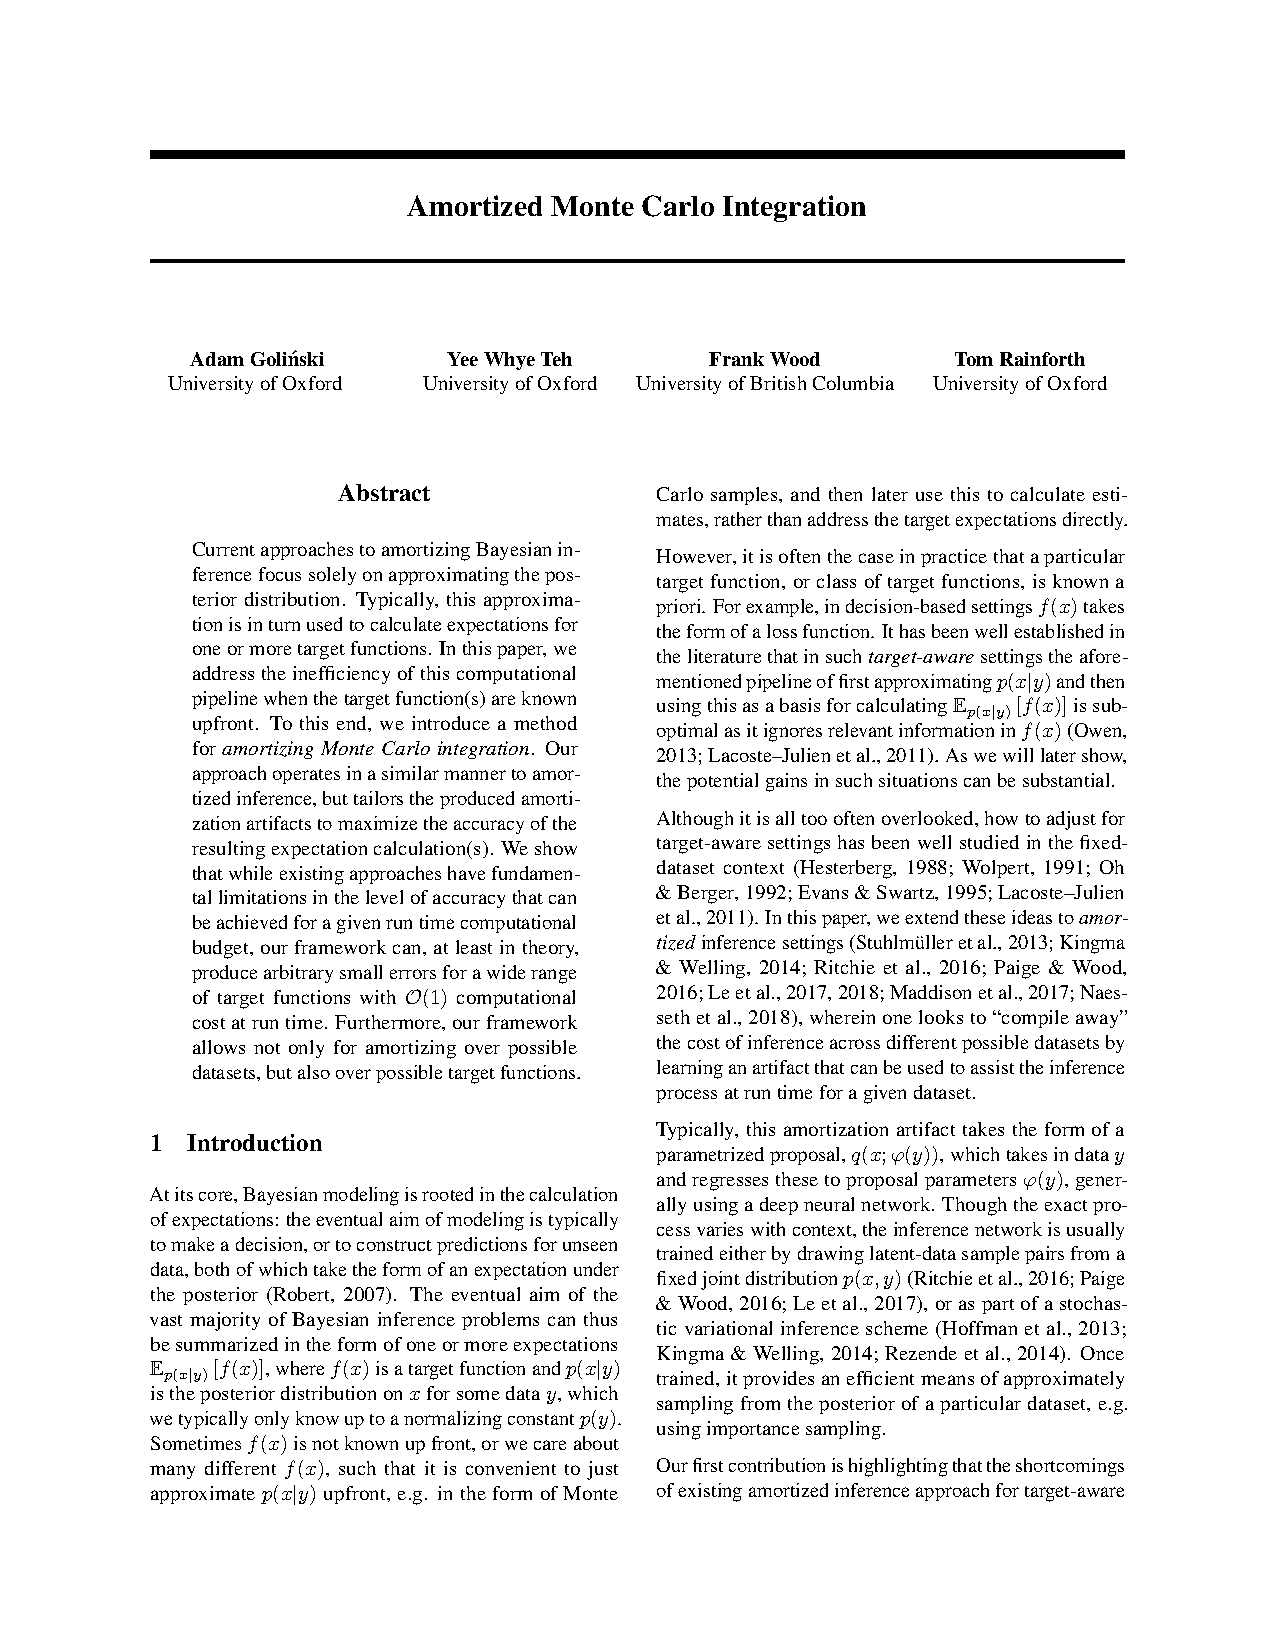
\includepdf[pages=-]{amci}


\end{document}
